\documentclass{standalone}

\usepackage{tikz}
\usetikzlibrary{arrows}
\usetikzlibrary{decorations.markings}
\usetikzlibrary{calc}

\begin{document}

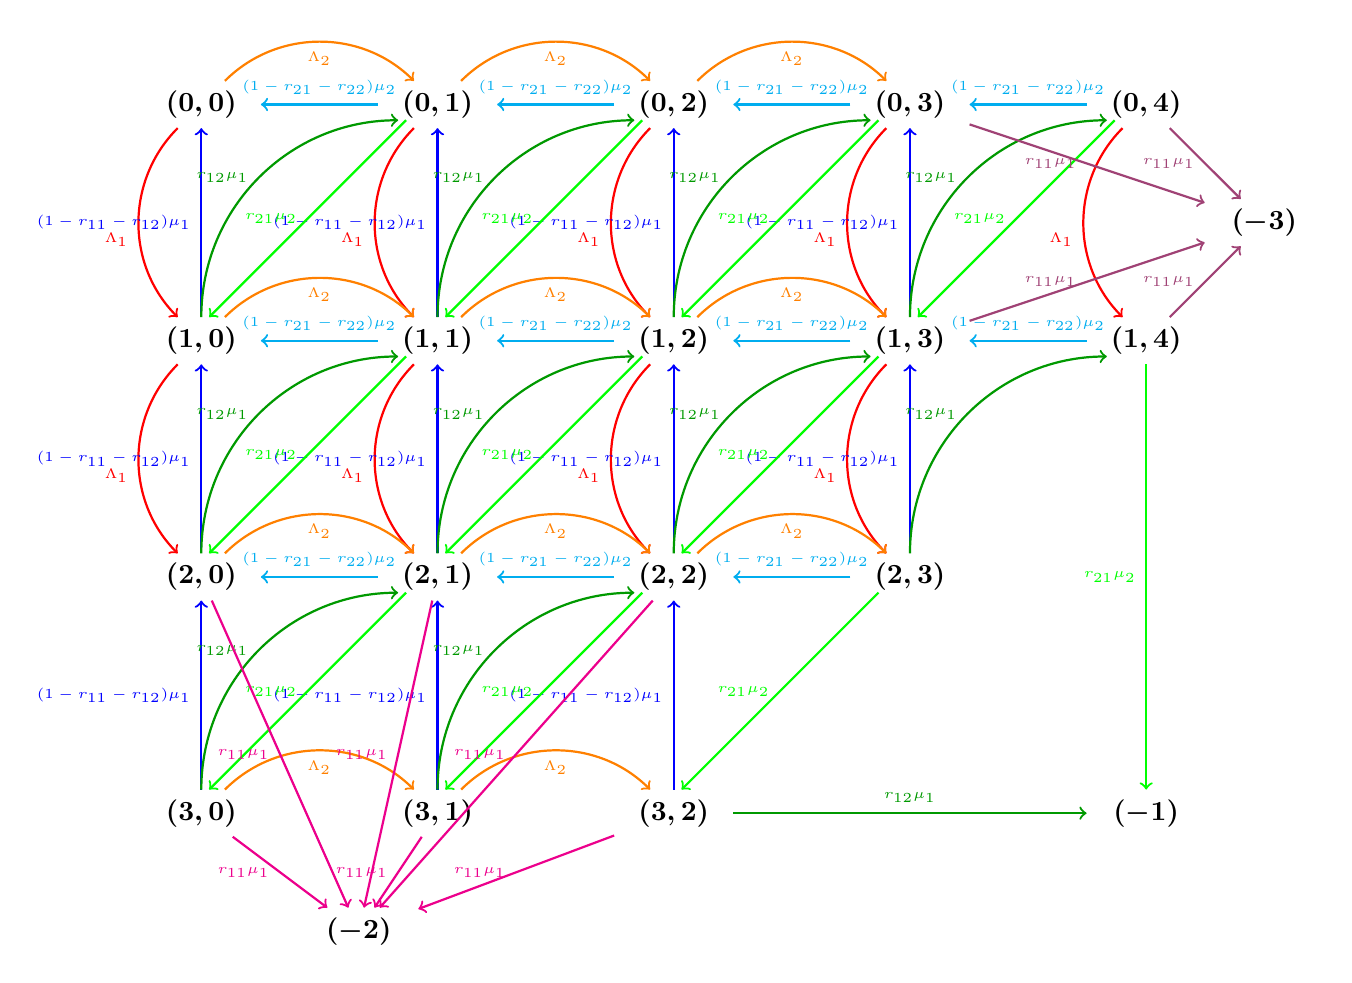
\begin{tikzpicture}
    \tikzstyle{state}=[minimum width=1.5cm, font=\boldmath];
    % First row
    \node (00) at (0,0) [state] {$(0,0)$};
    \node (01) at ($(00)+(3,0)$) [state] {$(0,1)$};
    \node (02) at ($(01)+(3,0)$) [state] {$(0,2)$};
    \node (03) at ($(02)+(3,0)$) [state] {$(0,3)$};
    \node (04) at ($(03)+(3,0)$) [state] {$(0,4)$};

    % Second row
    \node (10) at ($(00)+(0,-3)$) [state] {$(1,0)$};
    \node (11) at ($(10)+(3,0)$) [state] {$(1,1)$};
    \node (12) at ($(11)+(3,0)$) [state] {$(1,2)$};
    \node (13) at ($(12)+(3,0)$) [state] {$(1,3)$};
    \node (14) at ($(13)+(3,0)$) [state] {$(1,4)$};

    % Third row
    \node (20) at ($(10)+(0,-3)$) [state] {$(2,0)$};
    \node (21) at ($(20)+(3,0)$) [state] {$(2,1)$};
    \node (22) at ($(21)+(3,0)$) [state] {$(2,2)$};
    \node (23) at ($(22)+(3,0)$) [state] {$(2,3)$};

    % Fourth row
    \node (30) at ($(20)+(0,-3)$) [state] {$(3,0)$};
    \node (31) at ($(30)+(3,0)$) [state] {$(3,1)$};
    \node (32) at ($(31)+(3,0)$) [state] {$(3,2)$};

    \node (-1) at ($(32)+(6,0)$) [state] {$(-1)$};
    \node (-2) at ($(30)+(2,-1.5)$) [state] {$(-2)$};
    \node (-3) at ($(04)+(1.5,-1.5)$) [state] {$(-3)$};

    % Transitions
    % Arrivals
    \draw[draw=red] (00) edge[out=-135,in=135,->,thick] node [below left, text=red] {\tiny$\Lambda_1$} (10);
    \draw[draw=red] (01) edge[out=-135,in=135,->,thick] node [below left, text=red] {\tiny$\Lambda_1$} (11);
    \draw[draw=red] (02) edge[out=-135,in=135,->,thick] node [below left, text=red] {\tiny$\Lambda_1$} (12);
    \draw[draw=red] (03) edge[out=-135,in=135,->,thick] node [below left, text=red] {\tiny$\Lambda_1$} (13);
    \draw[draw=red] (04) edge[out=-135,in=135,->,thick] node [below left, text=red] {\tiny$\Lambda_1$} (14);

    \draw[draw=red] (10) edge[out=-135,in=135,->,thick] node [below left, text=red] {\tiny$\Lambda_1$} (20);
    \draw[draw=red] (11) edge[out=-135,in=135,->,thick] node [below left, text=red] {\tiny$\Lambda_1$} (21);
    \draw[draw=red] (12) edge[out=-135,in=135,->,thick] node [below left, text=red] {\tiny$\Lambda_1$} (22);
    \draw[draw=red] (13) edge[out=-135,in=135,->,thick] node [below left, text=red] {\tiny$\Lambda_1$} (23);

    \draw[draw=orange] (00) edge[out=45,in=135,->,thick] node [below, text=orange] {\tiny$\Lambda_2$} (01);
    \draw[draw=orange] (01) edge[out=45,in=135,->,thick] node [below, text=orange] {\tiny$\Lambda_2$} (02);
    \draw[draw=orange] (02) edge[out=45,in=135,->,thick] node [below, text=orange] {\tiny$\Lambda_2$} (03);

    \draw[draw=orange] (10) edge[out=45,in=135,->,thick] node [below, text=orange] {\tiny$\Lambda_2$}  (11);
    \draw[draw=orange] (11) edge[out=45,in=135,->,thick] node [below, text=orange] {\tiny$\Lambda_2$} (12);
    \draw[draw=orange] (12) edge[out=45,in=135,->,thick] node [below, text=orange] {\tiny$\Lambda_2$} (13);

    \draw[draw=orange] (20) edge[out=45,in=135,->,thick] node [below, text=orange] {\tiny$\Lambda_2$}  (21);
    \draw[draw=orange] (21) edge[out=45,in=135,->,thick] node [below, text=orange] {\tiny$\Lambda_2$} (22);
    \draw[draw=orange] (22) edge[out=45,in=135,->,thick] node [below, text=orange] {\tiny$\Lambda_2$} (23);

    \draw[draw=orange] (30) edge[out=45,in=135,->,thick] node [below, text=orange] {\tiny$\Lambda_2$}  (31);
    \draw[draw=orange] (31) edge[out=45,in=135,->,thick] node [below, text=orange] {\tiny$\Lambda_2$} (32);

    % % First Station Service and exit
    \draw[blue] (00) edge[<-,thick] node [left] {\tiny$(1-r_{11}-r_{12})\mu_1$} (10);
    \draw[blue] (01) edge[<-,thick] node [left] {\tiny$(1-r_{11}-r_{12})\mu_1$} (11);
    \draw[blue] (02) edge[<-,thick] node [left] {\tiny$(1-r_{11}-r_{12})\mu_1$} (12);
    \draw[blue] (03) edge[<-,thick] node [left] {\tiny$(1-r_{11}-r_{12})\mu_1$} (13);

    \draw[blue] (10) edge[<-,thick] node [left] {\tiny$(1-r_{11}-r_{12})\mu_1$} (20);
    \draw[blue] (11) edge[<-,thick] node [left] {\tiny$(1-r_{11}-r_{12})\mu_1$} (21);
    \draw[blue] (12) edge[<-,thick] node [left] {\tiny$(1-r_{11}-r_{12})\mu_1$} (22);
    \draw[blue] (13) edge[<-,thick] node [left] {\tiny$(1-r_{11}-r_{12})\mu_1$} (23);

    \draw[blue] (20) edge[<-,thick] node [left] {\tiny$(1-r_{11}-r_{12})\mu_1$} (30);
    \draw[blue] (21) edge[<-,thick] node [left] {\tiny$(1-r_{11}-r_{12})\mu_1$} (31);
    \draw[blue] (22) edge[<-,thick] node [left] {\tiny$(1-r_{11}-r_{12})\mu_1$} (32);

    % Second station service and exit
    \draw[draw=cyan] (04) edge[->,thick] node [above, text=cyan] {\tiny$(1-r_{21}-r_{22})\mu_2$} (03);
    \draw[draw=cyan] (03) edge[->,thick] node [above, text=cyan] {\tiny$(1-r_{21}-r_{22})\mu_2$} (02);
    \draw[draw=cyan] (02) edge[->,thick] node [above, text=cyan] {\tiny$(1-r_{21}-r_{22})\mu_2$} (01);
    \draw[draw=cyan] (01) edge[->,thick] node [above, text=cyan] {\tiny$(1-r_{21}-r_{22})\mu_2$} (00);

    \draw[draw=cyan] (14) edge[->,thick] node [above, text=cyan] {\tiny$(1-r_{21}-r_{22})\mu_2$} (13);
    \draw[draw=cyan] (13) edge[->,thick] node [above, text=cyan] {\tiny$(1-r_{21}-r_{22})\mu_2$} (12);
    \draw[draw=cyan] (12) edge[->,thick] node [above, text=cyan] {\tiny$(1-r_{21}-r_{22})\mu_2$} (11);
    \draw[draw=cyan] (11) edge[->,thick] node [above, text=cyan] {\tiny$(1-r_{21}-r_{22})\mu_2$} (10);

    \draw[draw=cyan] (23) edge[->,thick] node [above, text=cyan] {\tiny$(1-r_{21}-r_{22})\mu_2$} (22);
    \draw[draw=cyan] (22) edge[->,thick] node [above, text=cyan] {\tiny$(1-r_{21}-r_{22})\mu_2$} (21);
    \draw[draw=cyan] (21) edge[->,thick] node [above, text=cyan] {\tiny$(1-r_{21}-r_{22})\mu_2$} (20);

    % 1st station service and transition
    \draw[draw=green!60!black] (30) edge[out=90,in=180,->,thick] node [left, text=green!60!black] {\tiny$r_{12}\mu_1$} ($(21)+(-0.5,-0.2)$);
    \draw[draw=green!60!black] (20) edge[out=90,in=180,->,thick] node [left, text=green!60!black] {\tiny$r_{12}\mu_1$} ($(11)+(-0.5,-0.2)$);
    \draw[draw=green!60!black] (10) edge[out=90,in=180,->,thick] node [left, text=green!60!black] {\tiny$r_{12}\mu_1$} ($(01)+(-0.5,-0.2)$);

    \draw[draw=green!60!black] (31) edge[out=90,in=180,->,thick] node [left, text=green!60!black] {\tiny$r_{12}\mu_1$} ($(22)+(-0.5,-0.2)$);
    \draw[draw=green!60!black] (21) edge[out=90,in=180,->,thick] node [left, text=green!60!black] {\tiny$r_{12}\mu_1$} ($(12)+(-0.5,-0.2)$);
    \draw[draw=green!60!black] (11) edge[out=90,in=180,->,thick] node [left, text=green!60!black] {\tiny$r_{12}\mu_1$} ($(02)+(-0.5,-0.2)$);

    \draw[draw=green!60!black] (22) edge[out=90,in=180,->,thick] node [left, text=green!60!black] {\tiny$r_{12}\mu_1$} ($(13)+(-0.5,-0.2)$);
    \draw[draw=green!60!black] (12) edge[out=90,in=180,->,thick] node [left, text=green!60!black] {\tiny$r_{12}\mu_1$} ($(03)+(-0.5,-0.2)$);

    \draw[draw=green!60!black] (13) edge[out=90,in=180,->,thick] node [left, text=green!60!black] {\tiny$r_{12}\mu_1$} ($(04)+(-0.5,-0.2)$);
    \draw[draw=green!60!black] (23) edge[out=90,in=180,->,thick] node [left, text=green!60!black] {\tiny$r_{12}\mu_1$} ($(14)+(-0.5,-0.2)$);

    % 2ns station service and transition
    \draw[draw=green] ($(21)+(-0.4,-0.2)$) edge[->,thick] node [left, text=green] {\tiny$r_{21}\mu_2$} ($(30)+(0.1,0.3)$);
    \draw[draw=green] ($(11)+(-0.4,-0.2)$) edge[->,thick] node [left, text=green] {\tiny$r_{21}\mu_2$} ($(20)+(0.1,0.3)$);
    \draw[draw=green] ($(01)+(-0.4,-0.2)$) edge[->,thick] node [left, text=green] {\tiny$r_{21}\mu_2$} ($(10)+(0.1,0.3)$);

    \draw[draw=green] ($(22)+(-0.4,-0.2)$) edge[->,thick] node [left, text=green] {\tiny$r_{21}\mu_2$} ($(31)+(0.1,0.3)$);
    \draw[draw=green] ($(12)+(-0.4,-0.2)$) edge[->,thick] node [left, text=green] {\tiny$r_{21}\mu_2$} ($(21)+(0.1,0.3)$);
    \draw[draw=green] ($(02)+(-0.4,-0.2)$) edge[->,thick] node [left, text=green] {\tiny$r_{21}\mu_2$} ($(11)+(0.1,0.3)$);

    \draw[draw=green] ($(13)+(-0.4,-0.2)$) edge[->,thick] node [left, text=green] {\tiny$r_{21}\mu_2$} ($(22)+(0.1,0.3)$);
    \draw[draw=green] ($(03)+(-0.4,-0.2)$) edge[->,thick] node [left, text=green] {\tiny$r_{21}\mu_2$} ($(12)+(0.1,0.3)$);

    \draw[draw=green] ($(04)+(-0.4,-0.2)$) edge[->,thick] node [left, text=green] {\tiny$r_{21}\mu_2$} ($(13)+(0.1,0.3)$);
    \draw[draw=green] ($(23)+(-0.4,-0.2)$) edge[->,thick] node [left, text=green] {\tiny$r_{21}\mu_2$} ($(32)+(0.1,0.3)$);

    % To deadlock -1
    \draw[draw=green] (14) edge[->,thick] node [left, text=green] {\tiny$r_{21}\mu_2$} (-1);
    \draw[draw=green!60!black] (32) edge[->,thick] node [above, text=green!60!black] {\tiny$r_{12}\mu_1$} (-1);

    % To deadlock -2
    \draw[draw=magenta] (20) edge[->, thick] node [left, text=magenta] {\tiny$r_{11}\mu_1$} (-2);
    \draw[draw=magenta] (21) edge[->, thick] node [left, text=magenta] {\tiny$r_{11}\mu_1$} (-2);
    \draw[draw=magenta] (22) edge[->, thick] node [left, text=magenta] {\tiny$r_{11}\mu_1$} (-2);
    \draw[draw=magenta] (30) edge[->, thick] node [left, text=magenta] {\tiny$r_{11}\mu_1$} (-2);
    \draw[draw=magenta] (31) edge[->, thick] node [left, text=magenta] {\tiny$r_{11}\mu_1$} (-2);
    \draw[draw=magenta] (32) edge[->, thick] node [left, text=magenta] {\tiny$r_{11}\mu_1$} (-2);

    % TO deadlock -3
    \draw[draw=magenta!60!black] (03) edge[->, thick] node [left, text=magenta!60!black] {\tiny$r_{11}\mu_1$} (-3);
    \draw[draw=magenta!60!black] (04) edge[->, thick] node [left, text=magenta!60!black] {\tiny$r_{11}\mu_1$} (-3);
    \draw[draw=magenta!60!black] (13) edge[->, thick] node [left, text=magenta!60!black] {\tiny$r_{11}\mu_1$} (-3);
    \draw[draw=magenta!60!black] (14) edge[->, thick] node [left, text=magenta!60!black] {\tiny$r_{11}\mu_1$} (-3);



\end{tikzpicture}

\end{document}
